\section{Simulation Kinematic Variables Verification}\label{sec:analysis.simsmear.verify}

In the Sec.~\ref{sec:analysis.accept.verify} the simulation was verified for efficiency. Another systematic check on the simulation was performed to investigate the validity of the kinematic variables outputted from the simulation package~\ref{sec:analysis.simulation}. This procedure was also performed as a means to double check the conclusion about the simulation efficiency found in Sec.~\ref{sec:analysis.accept.verify} and to verify whether \abbr{GSIM} simulates \emph{pair-production} properly. To perform this check, first the total number of expected \piz events as well as $\pi^+\pi^-$ events were calculated for the beam energy range 1.1~GeV-2.8~GeV using the total cross-section, $\sigma$, for \piz and $\pi^+\pi^-$ production found in~\cite{durham} and using
\begin{align}
N_{events} = \sigma \rho L \ ,
\end{align}
where $\rho$ and $L$ are the target density and photon flux respectively. The total number of \piz and $\pi^+\pi^-$ events can be seen in Fig.~\ref{fig:simsmear.Ntot}, where the left axis depicts the number of \piz events and the right axis depicts the number of $\pi^+\pi^-$ events.
\begin{figure}[h!]\begin{center}
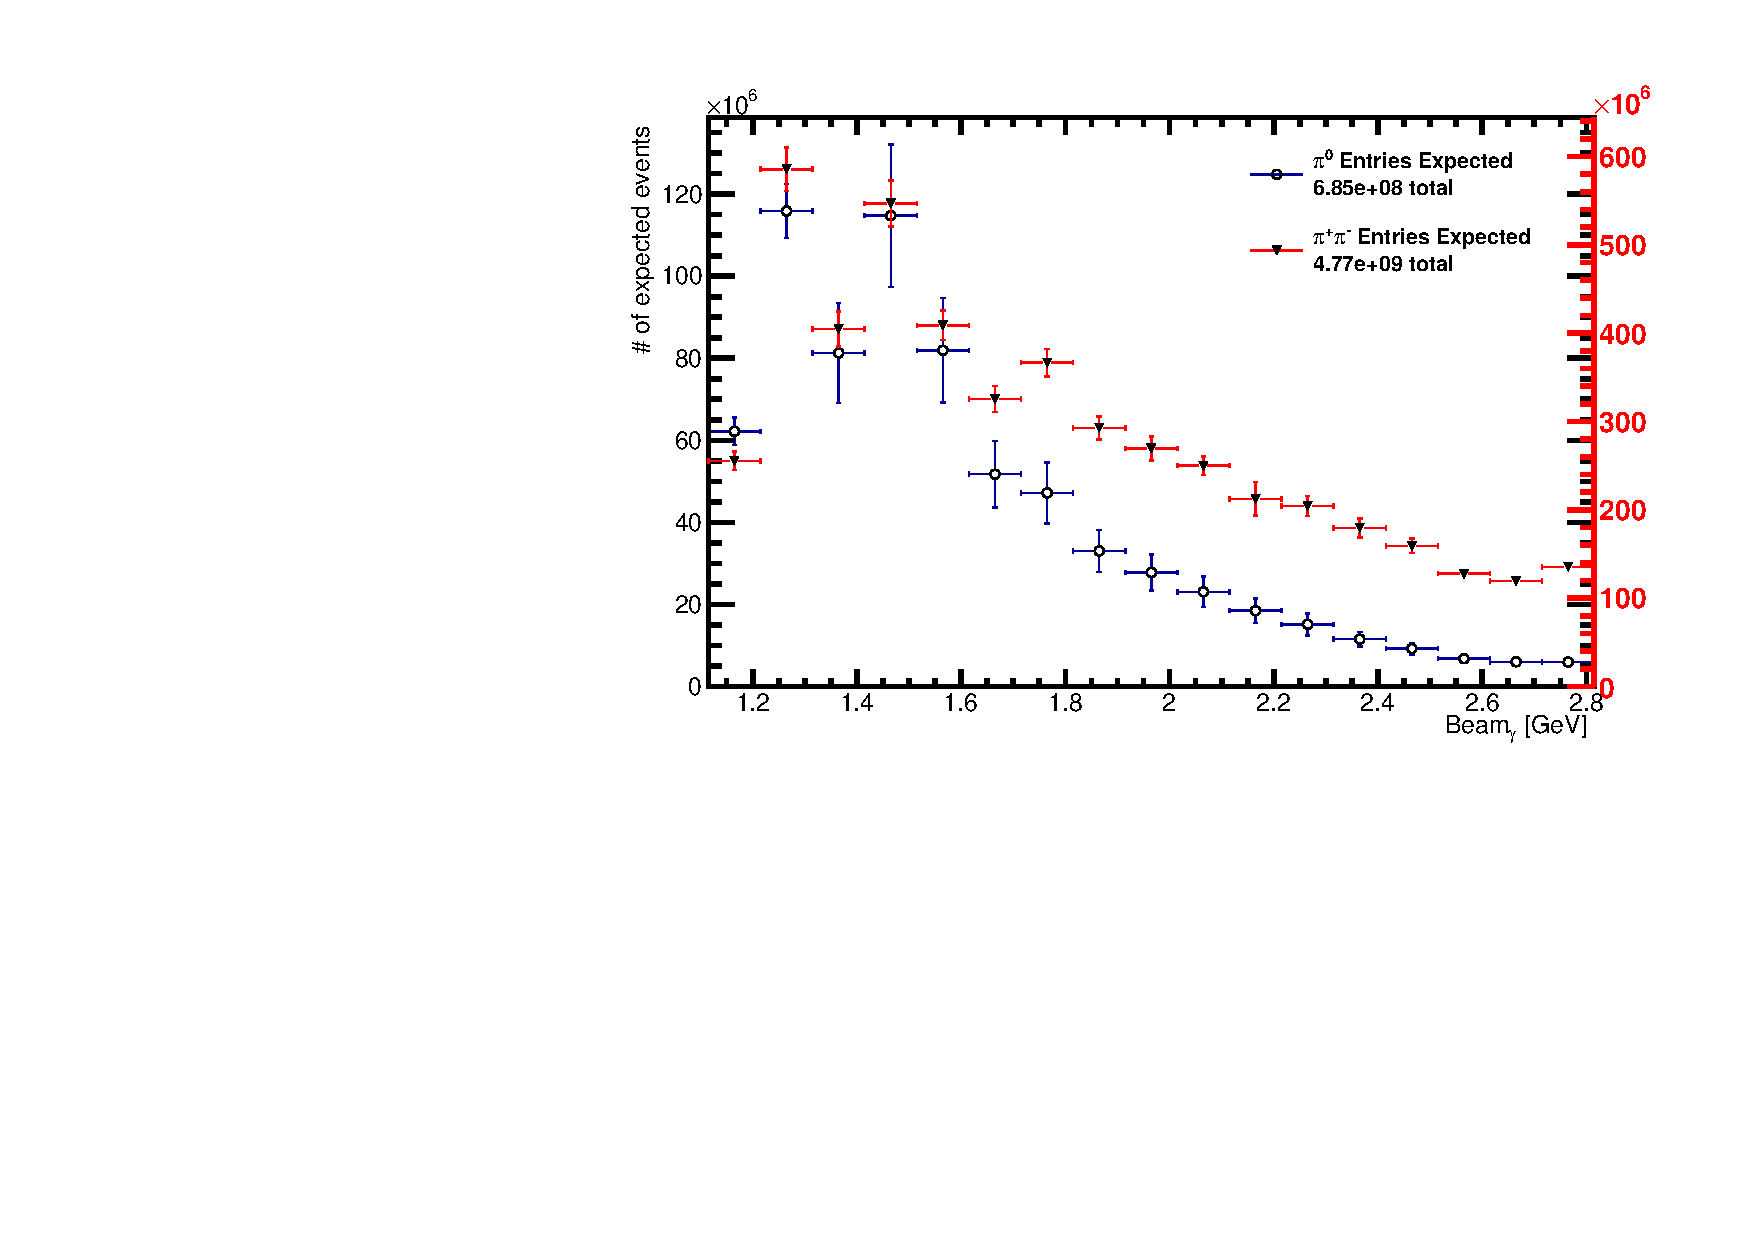
\includegraphics[width=\figwidth,height= 0.75 \hfigheight]{\figures/simulation/N_events.pdf}
\caption[Total Number of \piz and $\pi^+\pi^-$ Events Expected Between $E_{\gamma}$ 1.1~GeV-2.8~GeV ]{\label{fig:simsmear.Ntot}Total Number of \piz (black open circles) and $\pi^+\pi^-$ (black closed triangles) events expected between $E_{\gamma}$ 1.1~GeV-2.8~GeV. The left axis depicts the events expected for \piz production while the right axis depicts the events expected from $\pi^+\pi^-$ production. }
\end{center}\end{figure} 

Once the total amount of \piz was determined, it was necessary to determine the amount of \piz$\to \gamma \gamma$ and \piz $\to e^+e^- \gamma$ to generate. This was done via the branching ratios of \piz decay. The \piz $\to \gamma \gamma$ has a branching ratio of $98.823 \pm 0.034$\% while \piz$\to e^+e^- \gamma$ has a branching ratio of $1.174 \pm 0.035$\% ~\cite{pdg2014} which lead to $7.03914 \cdot10^8$ \piz $\to \gamma \gamma$ events generated and $8.36237 \cdot10^6$ \piz$\to e^+e^- \gamma$ events generated. Moreover, once the total amount of events were determined, the generation of the events was weighted using the \piz differential cross-section found in the SAID~\cite{SAID} database and the $\pi^+\pi^-$ differential cross-section found in the Durham~\cite{durham} database. After the events were generated, they were processed using the simulation package described in~\ref{sec:analysis.simulation} in which afterward were given the same fiducial cuts described in Sec.~\ref{sec:analysis.data.reduction}, kinematic constraint cuts Sec.~\ref{sec:analysis.fitting.compare} and trigger simulation cuts Sec.~\ref{sec:analysis.accept.trigger}. 

In Figs.~\ref{fig:simsmear.beam},~\ref{fig:simsmear.prot},~\ref{fig:simsmear.Ep},~\ref{fig:simsmear.Em} it is shown that the simulation procedure appears to give an accurate representation of physics events for the incident beam, detected proton positron and electron within \abbr{CLAS}. Furthermore, the overall acceptance and simulation of \emph{pair-production} is within a normalization factor of 1.011, meaning that the number of generated events was correct within 1.1\% or the simulation has an acceptance inefficiency of 1.1\%. The different sources contributing to the final detected \epem topology can be seen in Fig.~\ref{fig:simsmear.EpEm}. 

\begin{figure}[h!]\begin{center}
\subfloat[$\mathrm{M_x^2(p)}$ vs. $\mathrm{M_E^2(pe^+e^-)}$ for Data][]{ %Feynman diagram of \piz two photon decay
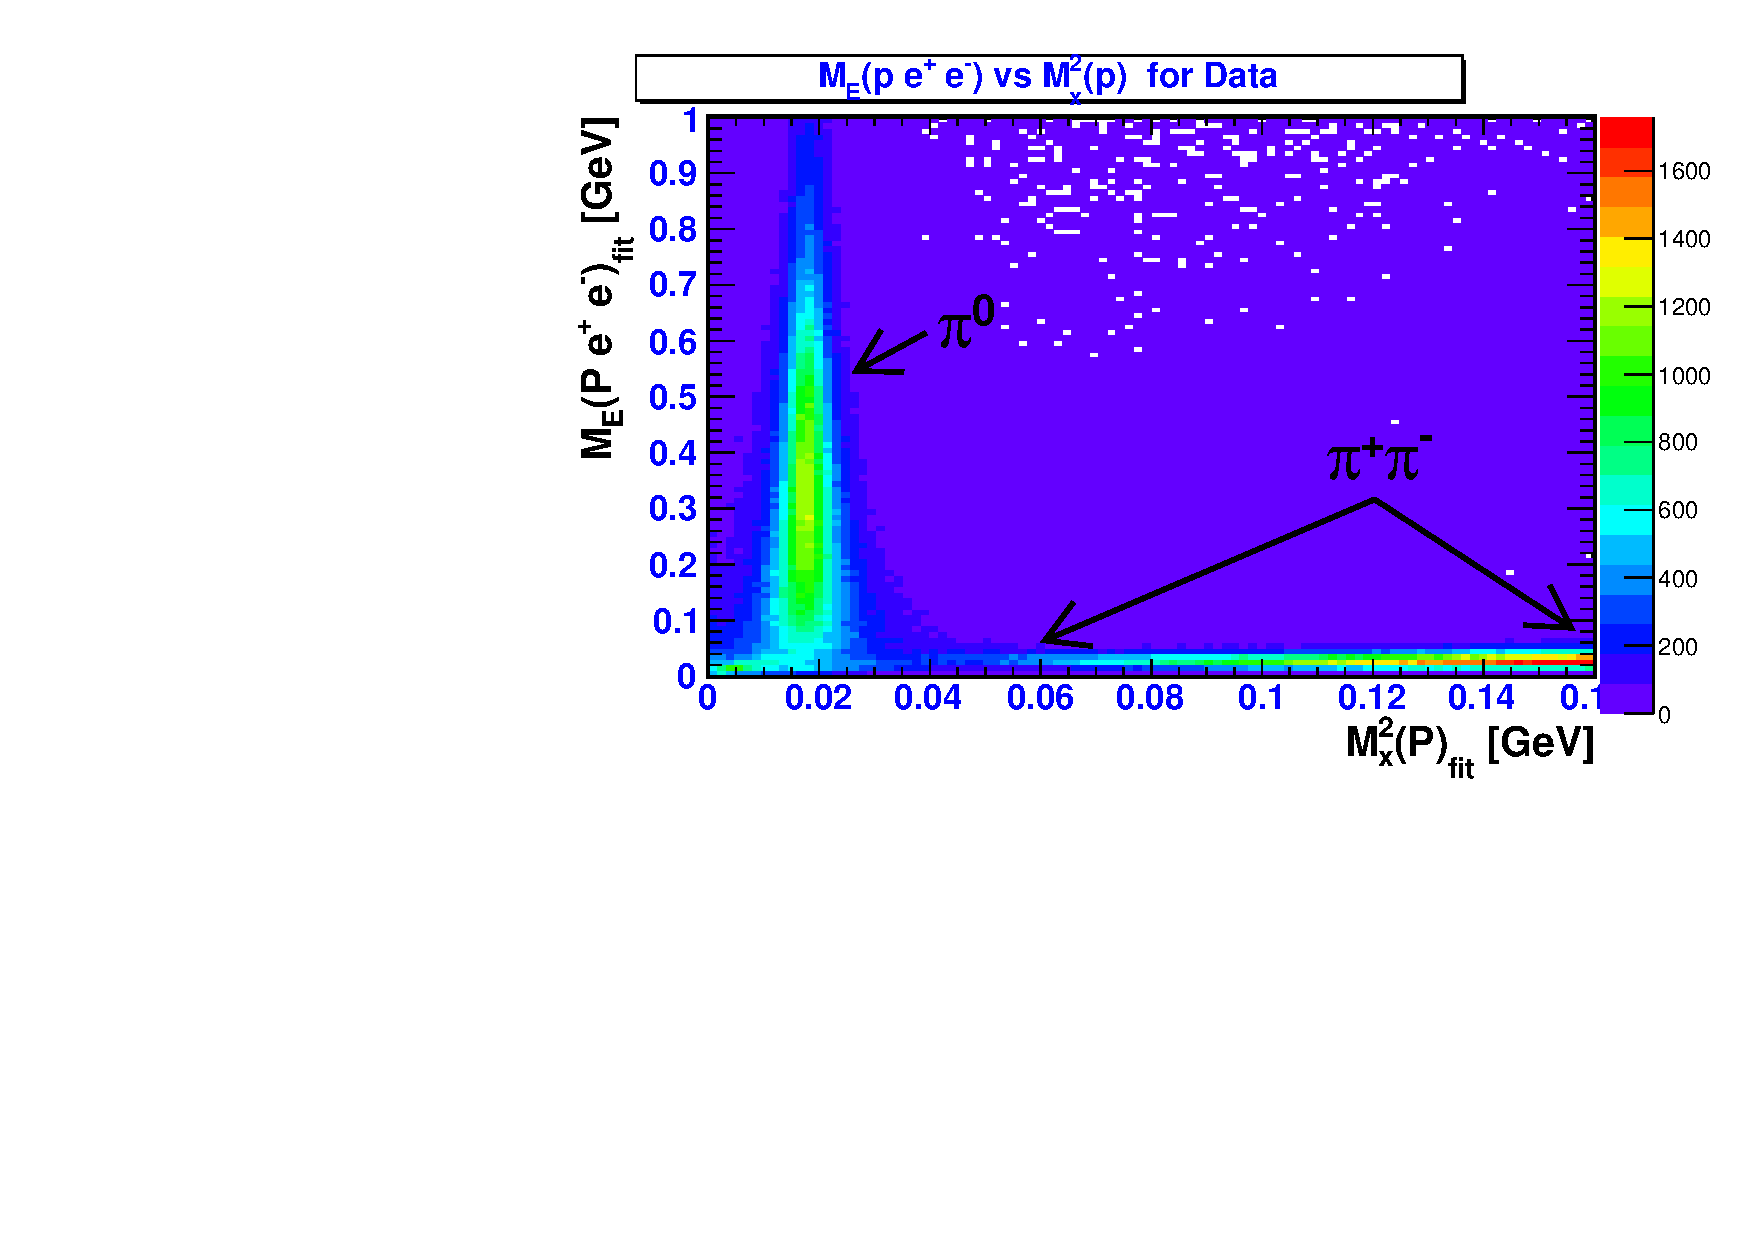
\includegraphics[width=\figwidth,height=\qfigheight]{\figures/simulation/ME_vs_MxP.pdf}\label{fig:simsmear.mEMxP.data}
}

\subfloat[$\mathrm{M_x^2(p)}$ vs. $\mathrm{M_E^2(pe^+e^-)}$ for \abbr{MC}]{ %Feynman diagram of \piz Dalitz decay
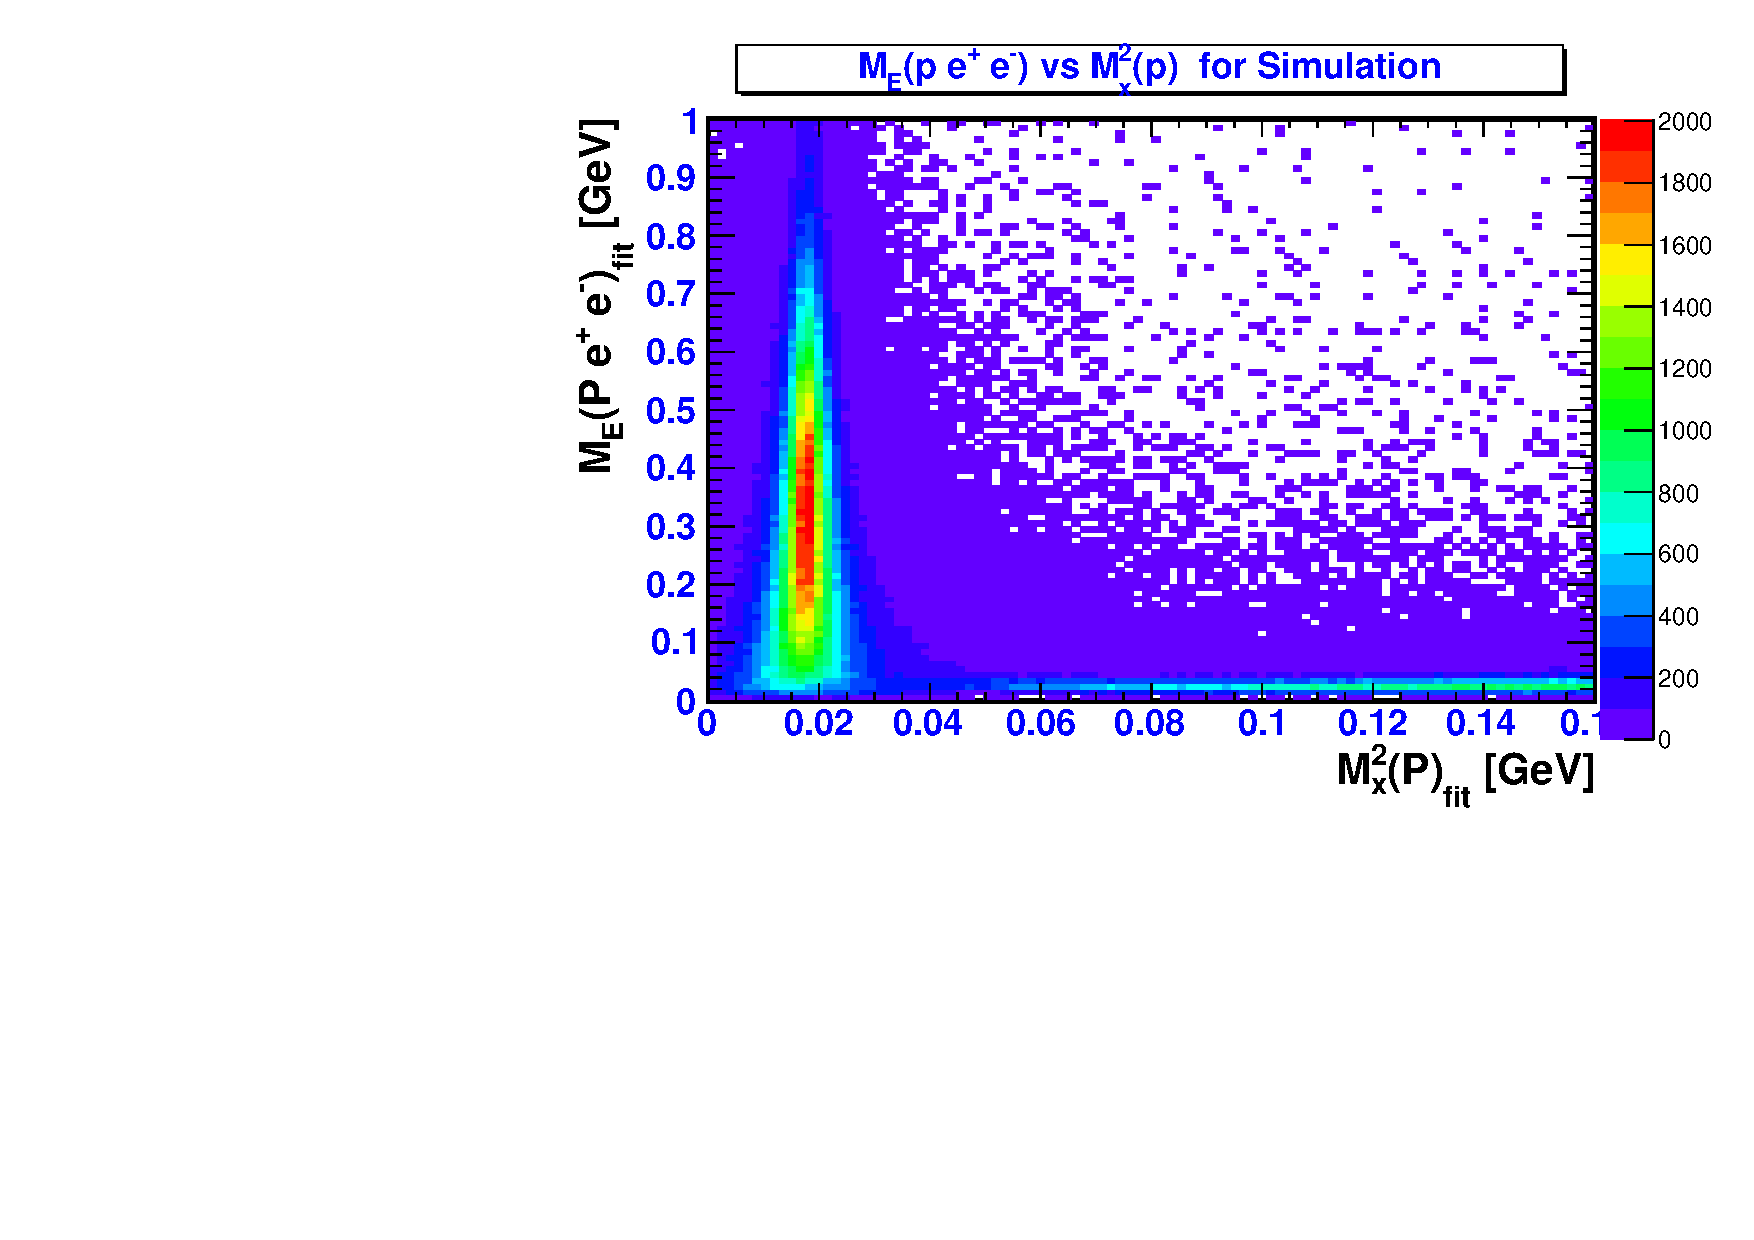
\includegraphics[width=0.8\columnwidth,height=\qfigheight]{\figures/simulation/ME_vs_MxP_simulation.pdf}\label{fig:simsmear.mEMxP.MC}
}
\caption[$\mathrm{M_x^2(\gamma p \to p X)}$ vs. $\mathrm{M_E^2(\gamma p \to pe^+e^- X)}$ for simulation systematic check]{\label{fig:simsmear.mEMxP.data.MC}$\mathrm{M_x^2(\gamma p \to p X)}$ vs. $\mathrm{M_E^2(\gamma p \to pe^+e^- X)}$ for simulation systematic check. Top panel depicts data, while the bottom panel depicts \abbr{MC}.}

\end{center}\end{figure}
%
%
\begin{figure}[h!]\begin{center}
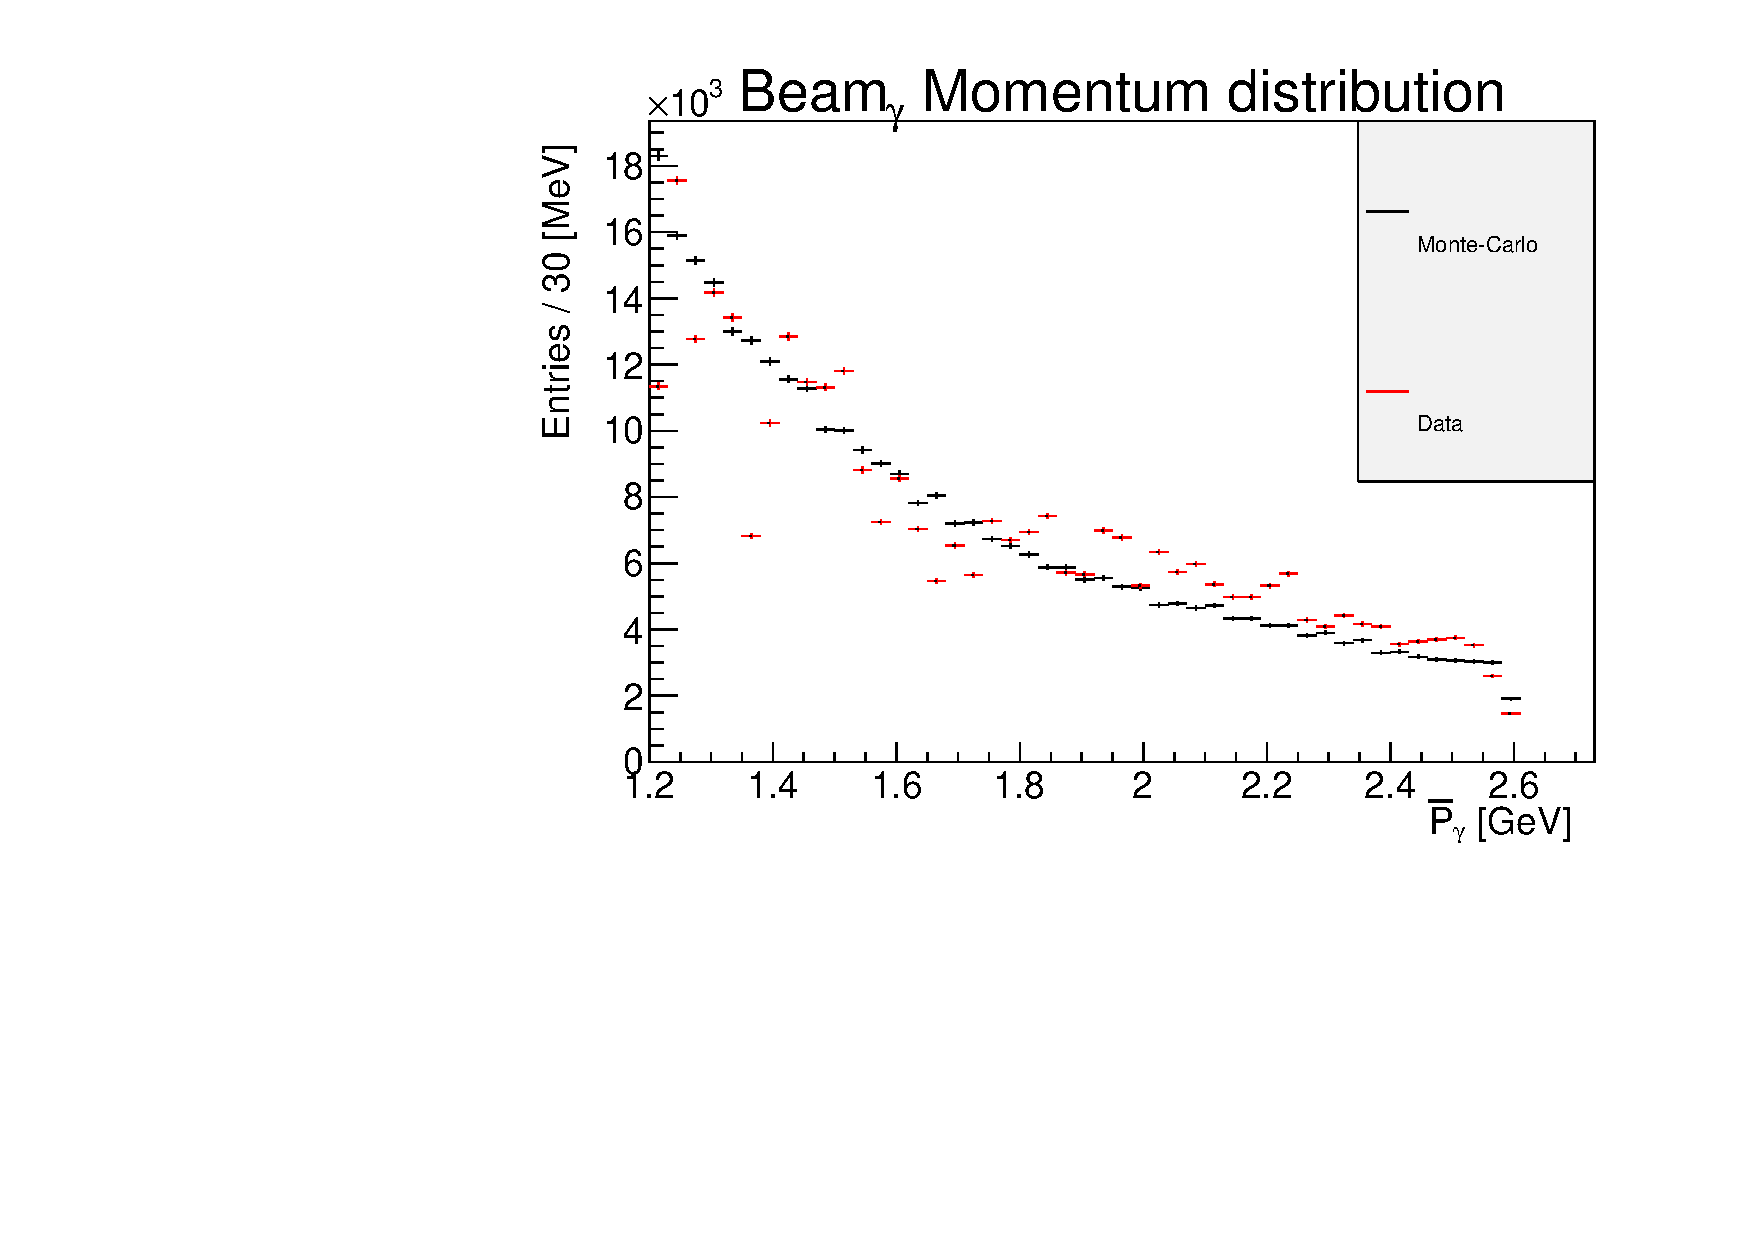
\includegraphics[width=\figwidth,height= 0.75 \hfigheight]{\figures/simulation/Beam_Kinematics_fitted.pdf}
\caption[Number of events vs. beam momentum for simulation systematic check]{\label{fig:simsmear.beam}Number of events vs. beam momentum for simulation systematic check. Comparison of incident photon beam kinematics for \abbr{MC} (black) events and data (red) when generating \abbr{MC} via differential cross-sections. Normalization factor is 1.011.}
\end{center}\end{figure} 
%
%
\begin{figure}[h!]\begin{center}
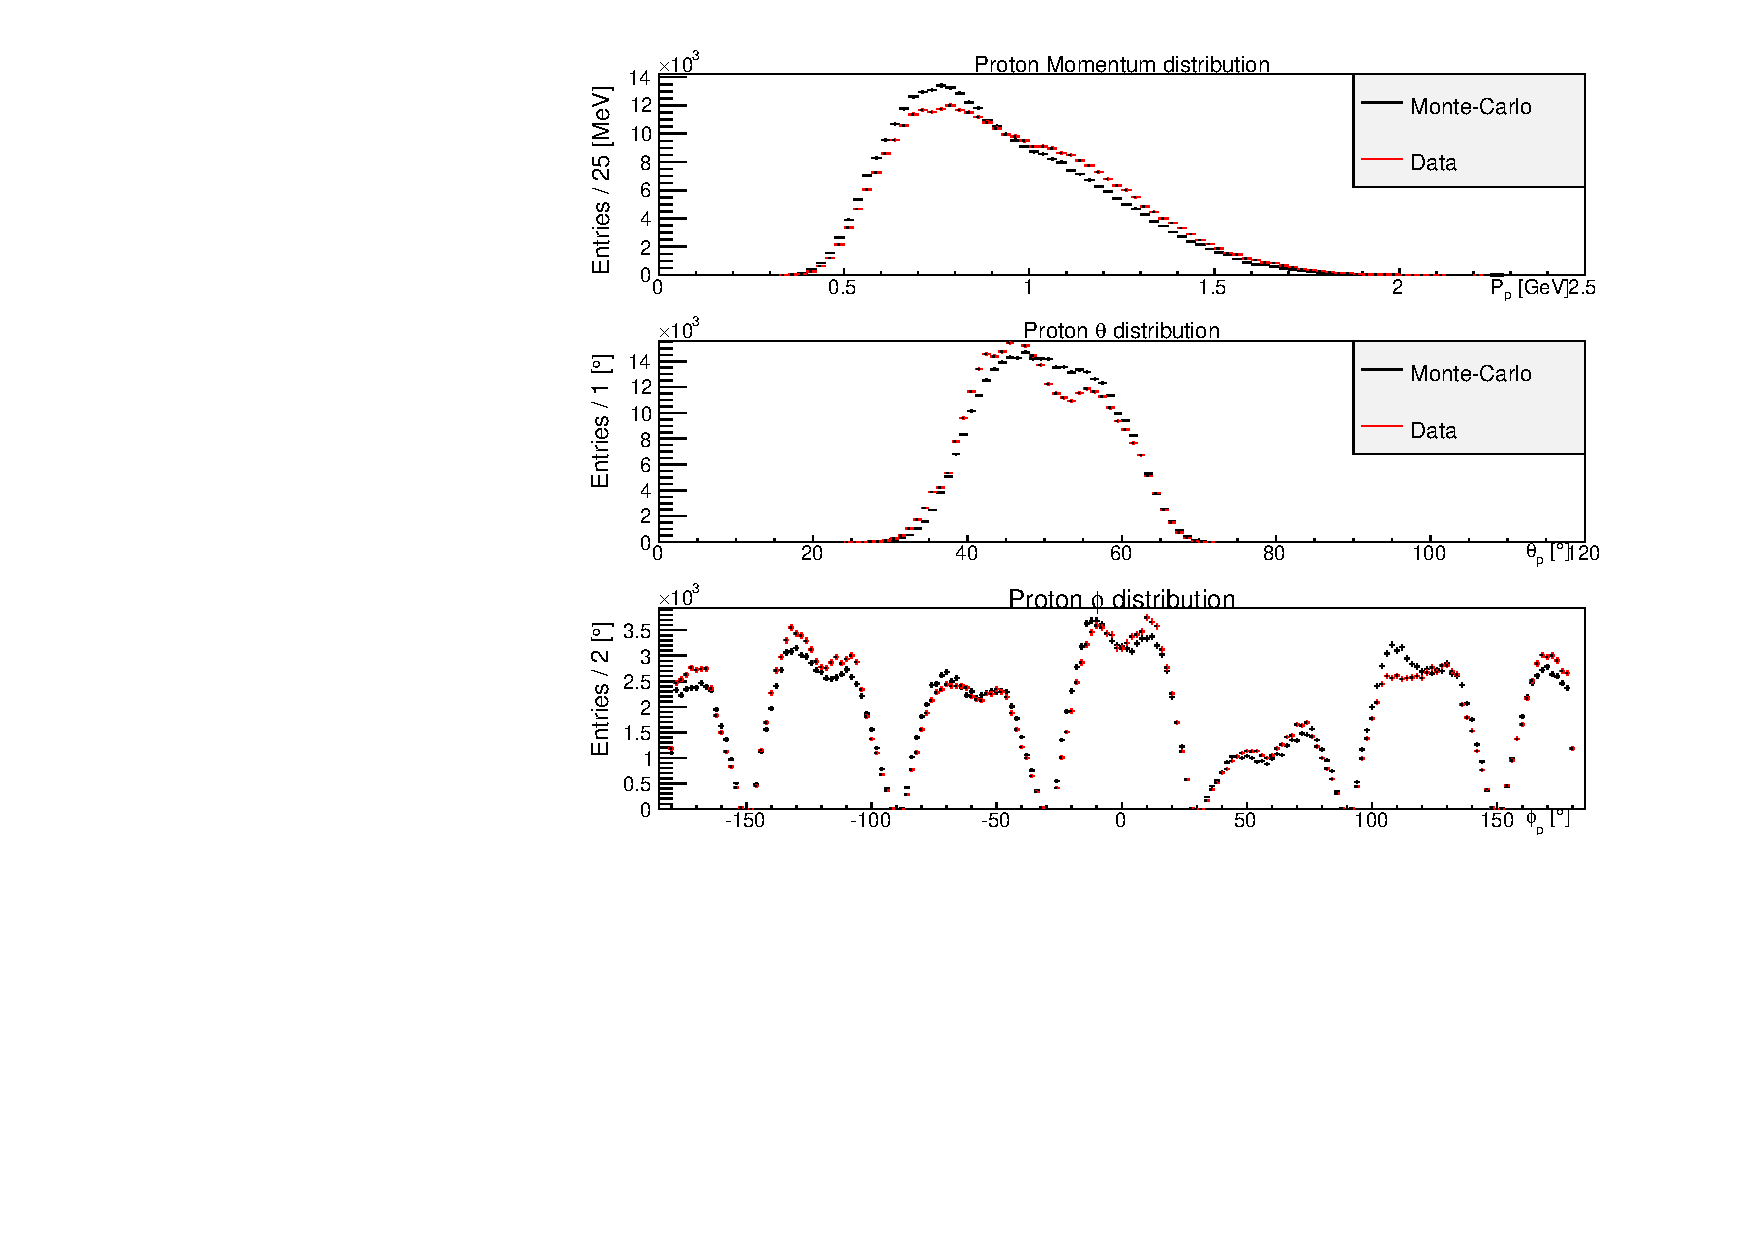
\includegraphics[width=\figwidth,height= 0.75 \hfigheight]{\figures/simulation/Proton_Kinematics_fitted.pdf}
\caption[Number of events vs. proton momentum (top), proton $\theta$ (middle) and proton $\phi$ kinematics for \abbr{MC} (black) events and data (red) when generating \abbr{MC} via differential cross-sections]{\label{fig:simsmear.prot}Number of events vs. proton momentum (top), proton $\theta$ (middle) and proton $\phi$ kinematics for \abbr{MC} (black) events and data (red) when generating \abbr{MC} via differential cross-sections. Normalization factor is 1.011. }
\end{center}\end{figure} 
%
%
\begin{figure}[h!]\begin{center}
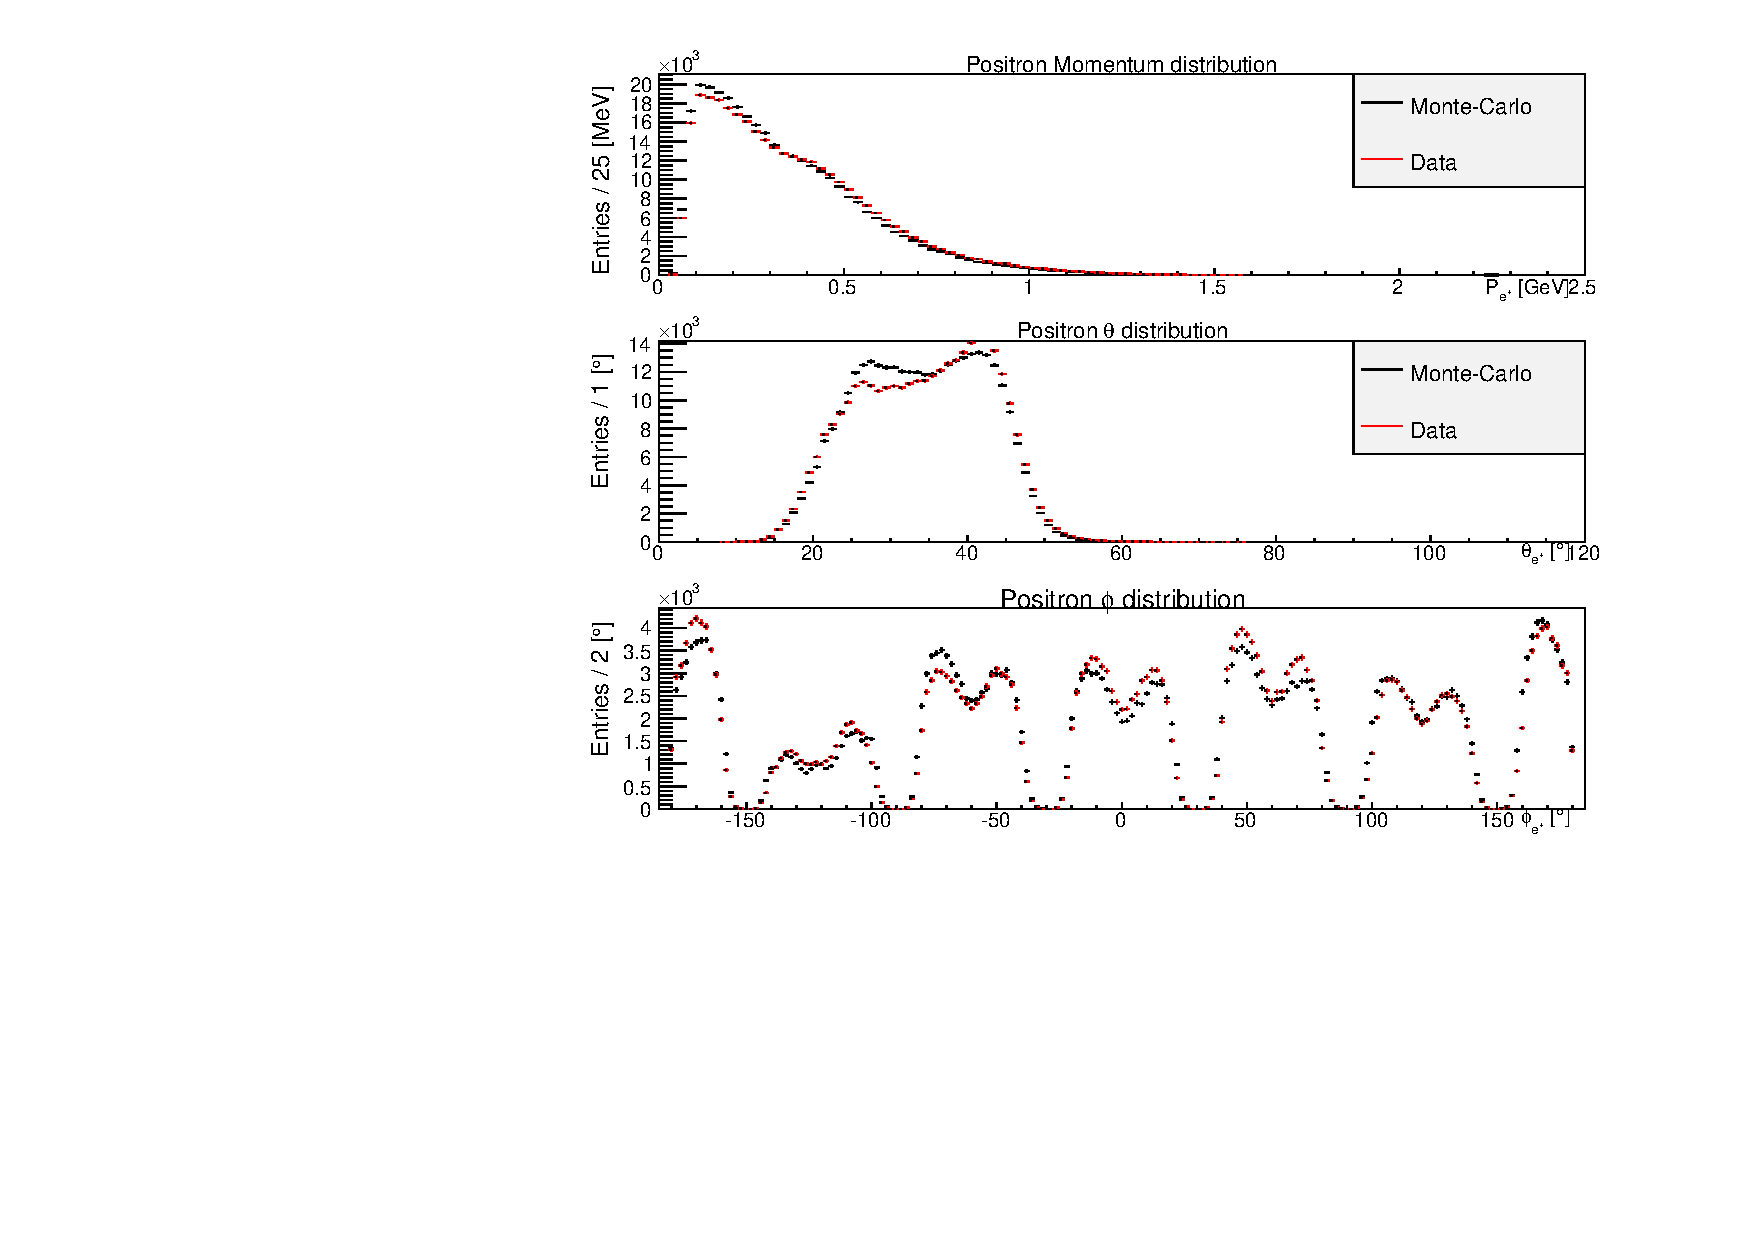
\includegraphics[width=\figwidth,height= 0.75 \hfigheight]{\figures/simulation/Positron_Kinematics_fitted.pdf}
\caption[Number of events vs. positron momentum (top), positron $\theta$ (middle) and positron $\phi$ kinematics for \abbr{MC} (black) events and data (red) when generating \abbr{MC} via differential cross-sections]{\label{fig:simsmear.Ep}Number of events vs. positron momentum (top), positron $\theta$ (middle) and positron $\phi$ kinematics for \abbr{MC} (black) events and data (red) when generating \abbr{MC} via differential cross-sections. Normalization factor is 1.011.}
\end{center}\end{figure} 
%
%
\begin{figure}[h!]\begin{center}
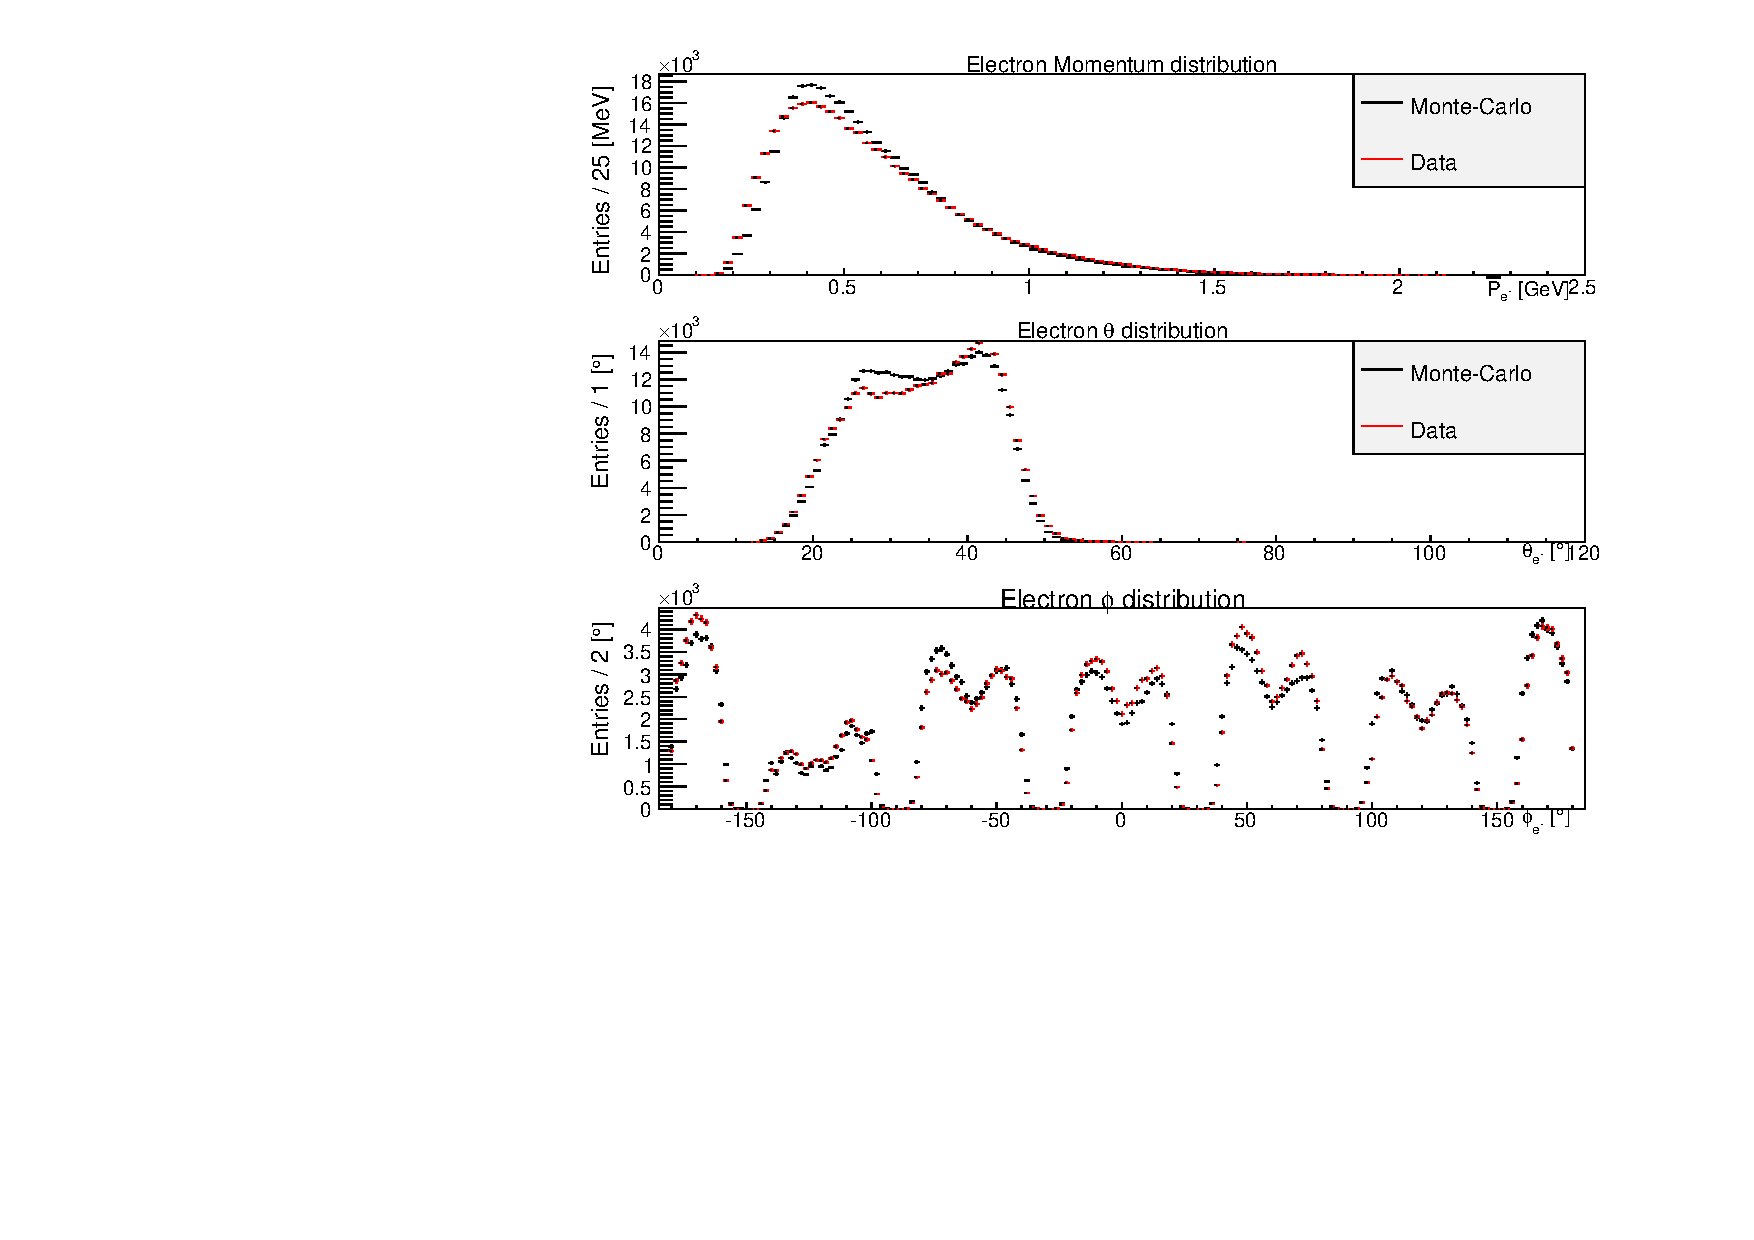
\includegraphics[width=\figwidth,height= 0.75 \hfigheight]{\figures/simulation/Electron_Kinematics_fitted.pdf}
\caption[Number of events vs. electron momentum (top), electron $\theta$ (middle) and electron $\phi$ kinematics for \abbr{MC} (black) events and data (red) when generating \abbr{MC} via differential cross-sections]{\label{fig:simsmear.Em}Number of events vs. electron momentum (top), electron $\theta$ (middle) and electron $\phi$ kinematics for \abbr{MC} (black) events and data (red) when generating \abbr{MC} via differential cross-sections. Normalization factor is 1.011. }
\end{center}\end{figure} 
%
%
\begin{figure}[h!]\begin{center}
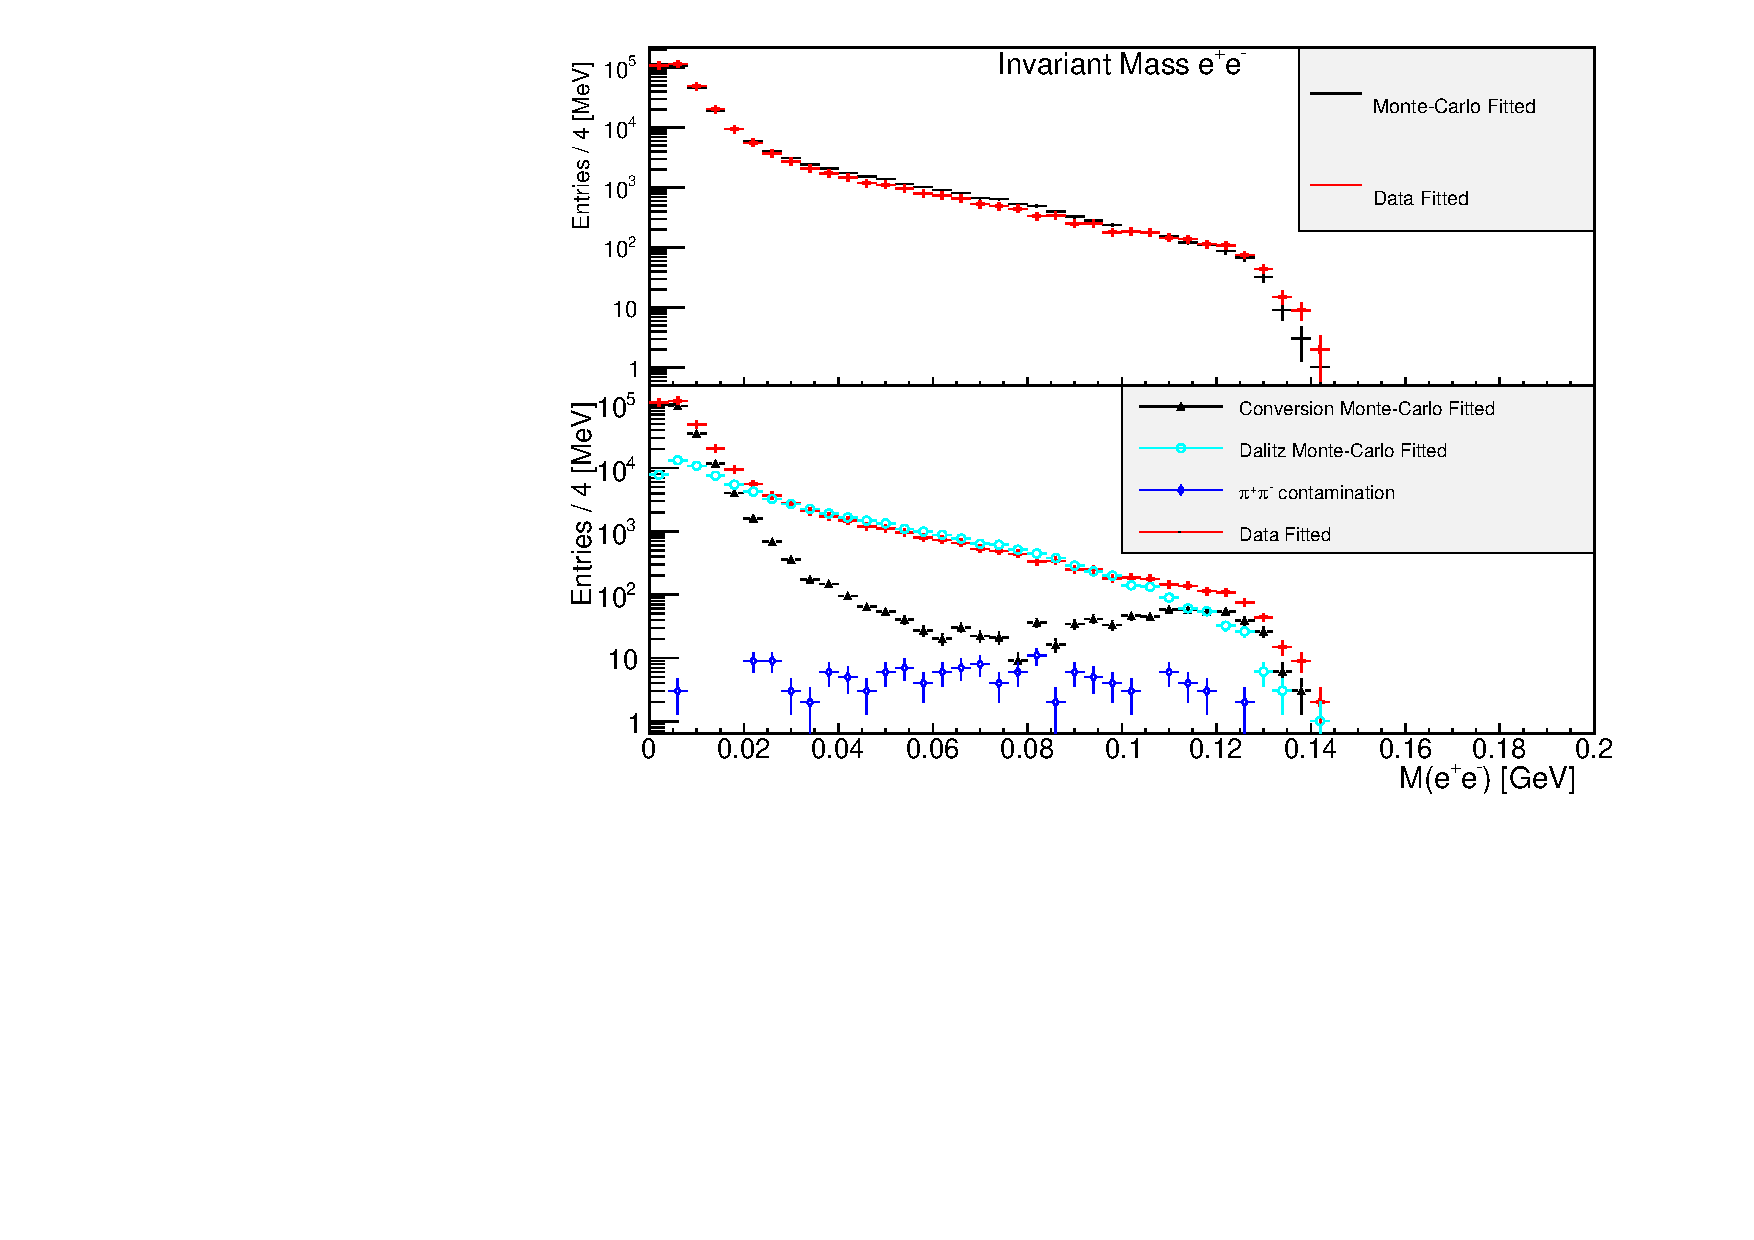
\includegraphics[width=\figwidth,height= 0.75 \hfigheight]{\figures/simulation/EpEm_Sources_fitted_combined.pdf}
\caption[Number of events vs. \epem mass distribution for all \abbr{MC} (black) events and data (red)]{\label{fig:simsmear.EpEm}Top Panel: Number of events vs. \epem mass distribution for all \abbr{MC} (black) events and data (red). Bottom Panel: Number of events vs. \epem mass distribution showing the sources of the \abbr{MC} \epem topology overlaid to the data. Normalization factor is 1.011.}
\end{center}\end{figure} 

\FloatBarrier
\section{Lepton Trigger Efficiency for \piz Candidates}\label{sec:analysis.trigger.verify}
Using all \piz candidates for incident beam energies less than 3.6~GeV, a trigger analysis was performed to investigate the lepton trigger ``bit 6'' efficiency. The normalization is the total number of \piz events as seen in the top panel of Fig.~\ref{fig:kinfit.final.plot} in Sec.~\ref{sec.final.data}. The normalization is done by calculating the total amount of entries for each trigger ``bit" and normalizing by the total amount of events. Since there was no heiarchy in the trigger configuration, a event can be triggered on multiple triggers. It can be seen in Fig~\ref{fig:Leptrigger} that for \piz candidates, below 3.6~GeV beam energy, the trigger ``bit 6'' efficiency is $\approx$100\%.

\begin{figure}[h!]\begin{center}
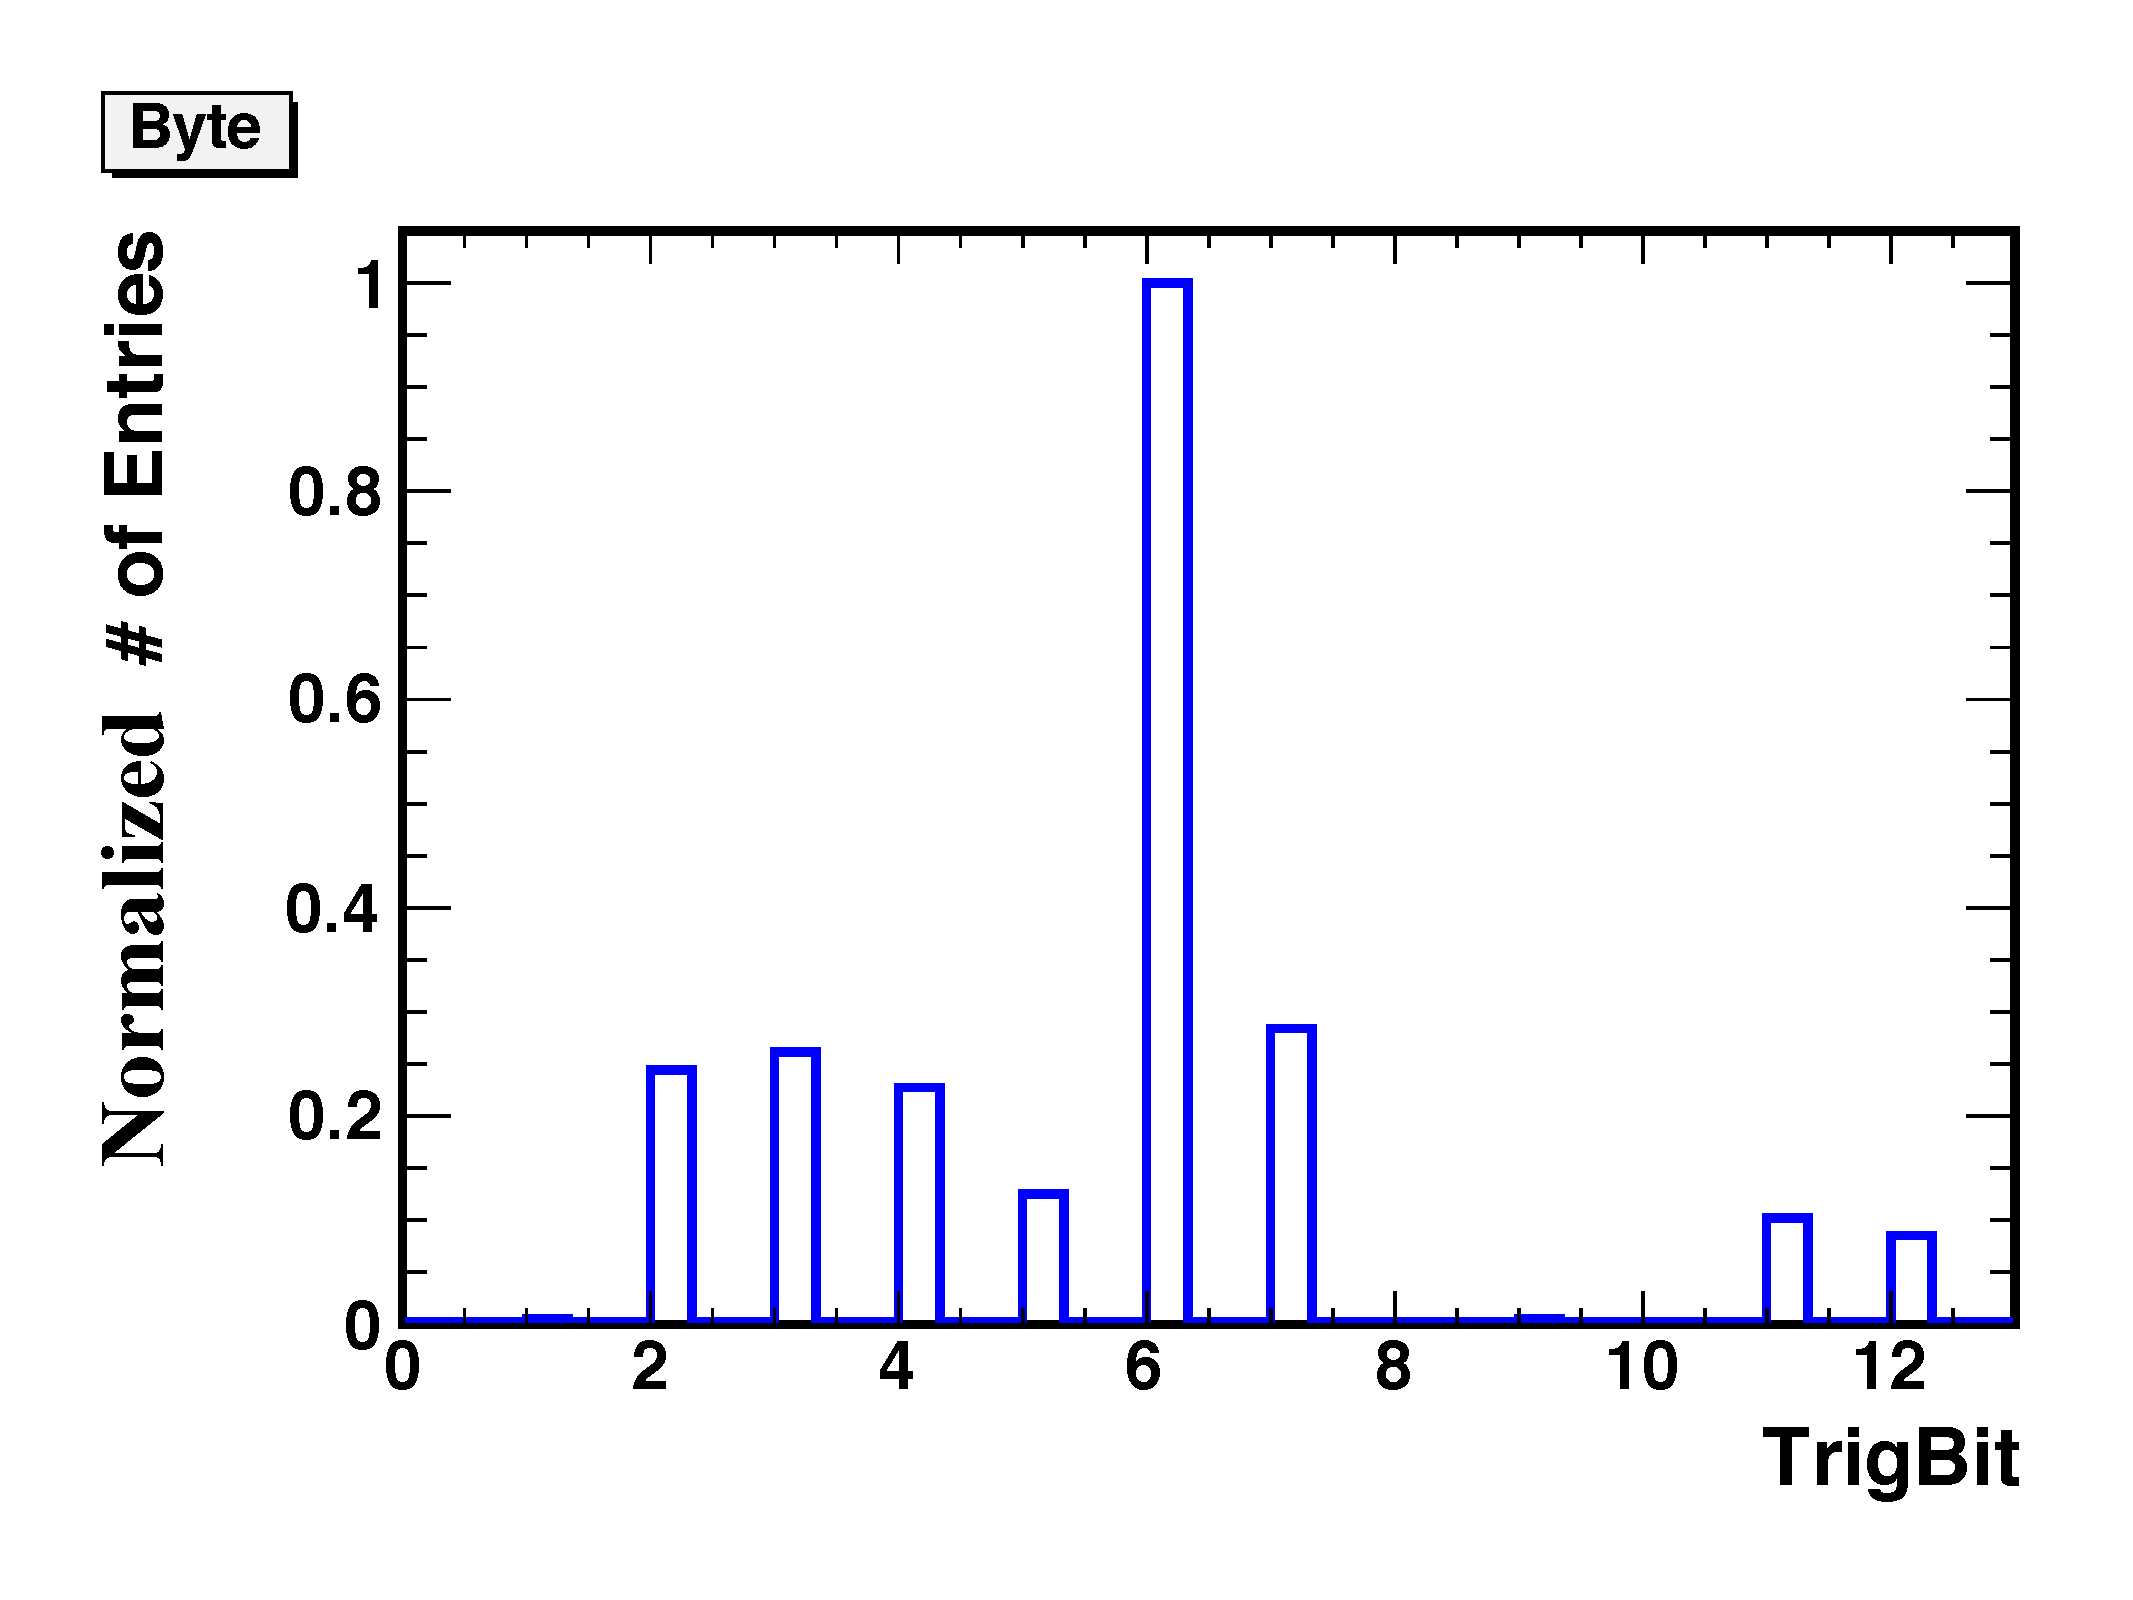
\includegraphics[width=\figwidth,height= 0.75 \hfigheight]{\figures/analysis/run57130_Twolep_normalizedII.pdf}
\caption[Normalized Lepton Trigger ``Bit 6'' for \piz candidates]{\label{fig:Leptrigger}Normalized lepton trigger ``bit 6'' for \piz candidates. The normalization is based upon the total number of \piz candidates.}
\end{center}\end{figure} 